\documentclass{beamer}

%\usepackage[table]{xcolor}
\mode<presentation> {
  \usetheme{Boadilla}
%  \usetheme{Pittsburgh}
%\usefonttheme[2]{sans}
\renewcommand{\familydefault}{cmss}
%\usepackage{lmodern}
%\usepackage[T1]{fontenc}
%\usepackage{palatino}
%\usepackage{cmbright}
  \setbeamercovered{transparent}
\useinnertheme{rectangles}
}
%\usepackage{normalem}{ulem}
%\usepackage{colortbl, textcomp}
\setbeamercolor{normal text}{fg = black}
\setbeamercolor{structure}{fg = blue}
\definecolor{trial}{cmyk}{1,0,0, 0}
\definecolor{trial2}{cmyk}{0.00,0,1, 0}
\definecolor{darkgreen}{rgb}{0,.4, 0.1}
\definecolor{mygray}{gray}{0.8}
\definecolor{myblack}{rgb}{0, 0, 0}
\usepackage{array}
\beamertemplatesolidbackgroundcolor{white}  \setbeamercolor{alerted
text}{fg=red}

\setbeamertemplate{caption}[numbered]\newcounter{mylastframe}

\usepackage{color}
\usepackage{tikz}
\usetikzlibrary{arrows}
\usepackage{colortbl}
\usepackage{graphicx}
\usepackage{epsfig}

%\usepackage[usenames, dvipsnames]{color}
%\setbeamertemplate{caption}[numbered]\newcounter{mylastframe}c
%\newcolumntype{Y}{\columncolor[cmyk]{0, 0, 1, 0}\raggedright}
%\newcolumntype{C}{\columncolor[cmyk]{1, 0, 0, 0}\raggedright}
%\newcolumntype{G}{\columncolor[rgb]{0, 1, 0}\raggedright}
%\newcolumntype{R}{\columncolor[rgb]{1, 0, 0}\raggedright}

%\begin{beamerboxesrounded}[upper=uppercol,lower=lowercol,shadow=true]{Block}
%$A = B$.
%\end{beamerboxesrounded}}
\renewcommand{\familydefault}{cmss}
%\usepackage[all]{xy}

\usepackage{tikz}
\usepackage{lipsum}

 \newenvironment{changemargin}[3]{%
 \begin{list}{}{%
 \setlength{\topsep}{0pt}%
 \setlength{\leftmargin}{#1}%
 \setlength{\rightmargin}{#2}%
 \setlength{\topmargin}{#3}%
 \setlength{\listparindent}{\parindent}%
 \setlength{\itemindent}{\parindent}%
 \setlength{\parsep}{\parskip}%
 }%
\item[]}{\end{list}}
\usetikzlibrary{arrows}
%\usepackage{palatino}
%\usepackage{eulervm}
\usecolortheme{lily}

\newtheorem{com}{Comment}
\newtheorem{lem} {Lemma}
\newtheorem{prop}{Proposition}
\newtheorem{thm}{Theorem}
\newtheorem{defn}{Definition}
\newtheorem{cor}{Corollary}
\newtheorem{obs}{Observation}
 \numberwithin{equation}{section}


\title[PLSC 43401] % (optional, nur bei langen Titeln nötig)
{Mathematical Foundations of Political Methodology}

\author{Robert Gulotty}
\institute[University of Chicago]{Associate Professor\\Department of Political Science \\  University of Chicago}
\vspace{0.3in}
\date{August 28th, 2017}

\setbeamertemplate{navigation symbols}{}

\begin{document}



\begin{frame}
\titlepage
\end{frame}



\begin{frame}

\begin{itemize}
\item \textcolor{myblack}{Integral}
\item \textcolor{myblack}{Fundamental Theorem of Calculus}
\item \textcolor{myblack}{Integration Facts}
\item \textcolor{myblack}{Indefinite and Definite Integrals}
\end{itemize}

\end{frame}



\begin{frame}

\begin{itemize}
\item \textcolor{myblack}{Integral}
\item \textcolor{mygray}{Fundamental Theorem of Calculus}
\item \textcolor{mygray}{Integration Facts}
\item \textcolor{mygray}{Indefinite and Definite Integrals}
\end{itemize}

\end{frame}



\begin{frame}
\frametitle{Integral: Geometric Intuitions}

``The opposite of differentiation," ``antiderivative," or ``taking an area"
 
\vspace{.2in}
\begin{center}
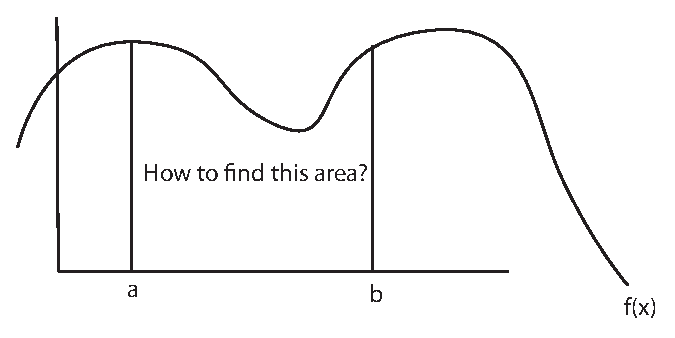
\epsfig{file=question.eps, scale=.7}
\end{center}
 
\end{frame}



\begin{frame}
\frametitle{Integral: Geometric Intuitions}

Let $a<b$ be real numbers and let $f$ be a continuous function. \pause
 
\ \\We want to find the area bounded by the curve $y=f(x)$, the vertical lines $x=a$ and $x=b$, and the $x$-axis.  Let $a=x_o$ and $b=x_7$

\begin{center}
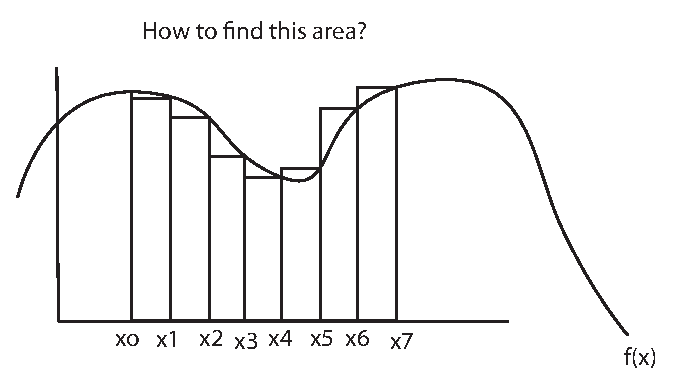
\epsfig{file=question2.eps, scale=.7}
\end{center}

\end{frame}



\begin{frame}
\frametitle{Integral: Geometric Intuitions}

\begin{center}
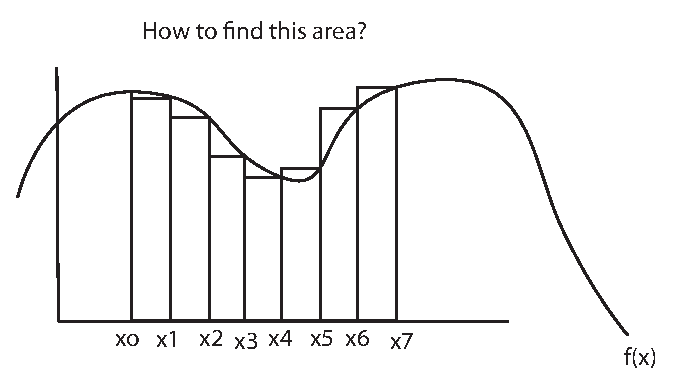
\epsfig{file=question2.eps, scale=.5}
\end{center}
  
$\sum_{i=1}^7 (x_i-x_{i-1})f(x_i)$  or letting $\Delta x_i=x_i-x_{i-1}$ this approximation is
$\sum_{i=1}^7 f(x_i) \Delta x_i$ \pause

\ \\Letting $\lim_{\Delta x_i}\rightarrow 0$ gives us the solution; it's written $$\int_a^b f(x) dx$$

\end{frame}



\begin{frame}
\frametitle{Integral: Geometric Intuitions}

Areas below the $x-$axis are negative: $$\int_a^b f(x)=\hbox{Area(A)-Area(B)}$$
  
\begin{center}
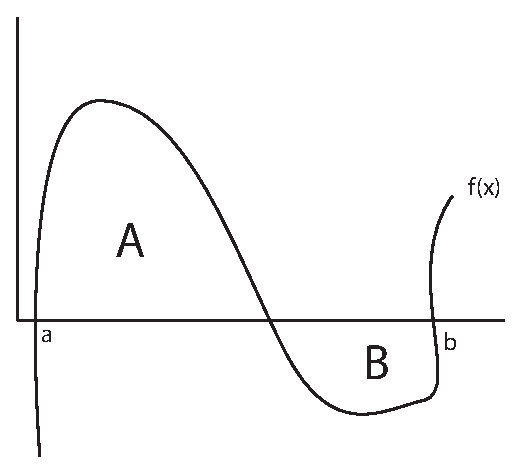
\epsfig{file=negative.eps, scale=.5}
\end{center}

\end{frame}



\begin{frame}
\frametitle{Integral: Definition}

\begin{defn} Suppose $f:\Re \rightarrow \Re$.  We will define the Riemann Integral as $\int_{a}^{b} f(x) dx$.  If this exists then we say $f$ is \alert{integrable} on $[a,b]$ and call $\int_{a}^{b} f(x) dx$ the \alert{integral} of f.  
\end{defn}

\end{frame}



\begin{frame}
\frametitle{Integral: Definition}

Suppose $f:[0,1]\rightarrow \frac{1}{x}$ 
\begin{eqnarray}
\int_{0}^{1} \frac{1}{x} dx \nonumber 
\end{eqnarray} \pause 

Then $\frac{1}{x}$ is not integrable on $[a,b]$ because the area that the integral would represent is infinite.  \pause \\ 

\begin{eqnarray}
f(x) & = & 1 \text{ if $x$ rational} \nonumber \\
	 & = & 0 \text{ if $x$ irrational} \nonumber 
\end{eqnarray} \pause 

This function is called Dirichlet Function, it is not integrable, because every interval will contain a discontinuous jump 

\end{frame}



\begin{frame}

\begin{itemize}
\item \textcolor{mygray}{Integral}
\item \textcolor{myblack}{Fundamental Theorem of Calculus}
\item \textcolor{mygray}{Integration Facts}
\item \textcolor{mygray}{Indefinite and Definite Integrals}
\end{itemize}

\end{frame}



\begin{frame}
\frametitle{Fundamental Theorem of Calculus}

There is a connection between derivative and integral, the relationship is descried by the Fundamental Theorem of Calculus. \pause Before we introduce the Fundamental Theorem of Calculus, we introduce following theorem.

\begin{theorem}
Given a number $a$ and a continuous function $f(x)$ we can define another function $F$ such that $$F(t)=\int_a^t f(x) dx \hbox{ for all } t$$
Then $F$ is differentiable and $F^\prime(t)=f(t)$ for all $t$
\end{theorem} \pause
 
\ \\If you integrate a function and then differentiate the result, you retrieve the function that you started with  $\Rightarrow$ ``integration is the reverse of differentiation"

\end{frame}



\begin{frame}
\frametitle{Fundamental Theorem of Calculus}

\begin{center}
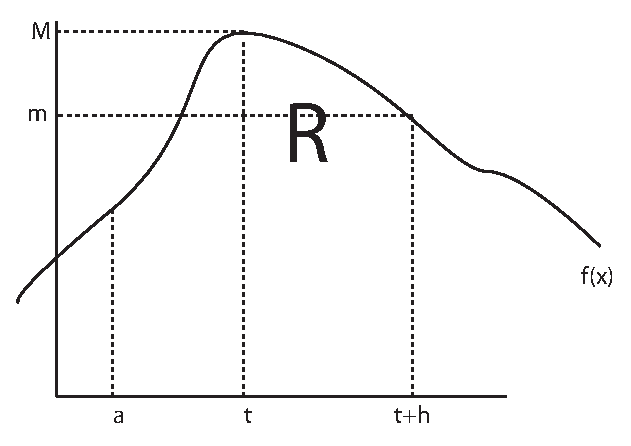
\epsfig{file=fundamental.eps, scale=.5}
\end{center}

Proof: Let $R=\int_t^{t+h}f(x) dx$ and let $F(t)=\int_a^t f(x) dx \hbox{ for all } t$. \pause Then $$R=\int_a^{t+h}f(x)dx-\int_a^{t}f(x)dx=F(t+h)-F(t)$$ \pause
We also have that $$ hm\leq F(t+h)-F(t)\leq hM, \hbox{ or }$$
$$m\leq \frac{F(t+h)-F(t)}{h}\leq M$$ 

\end{frame}



\begin{frame}
\frametitle{Fundamental Theorem of Calculus}

\begin{center}
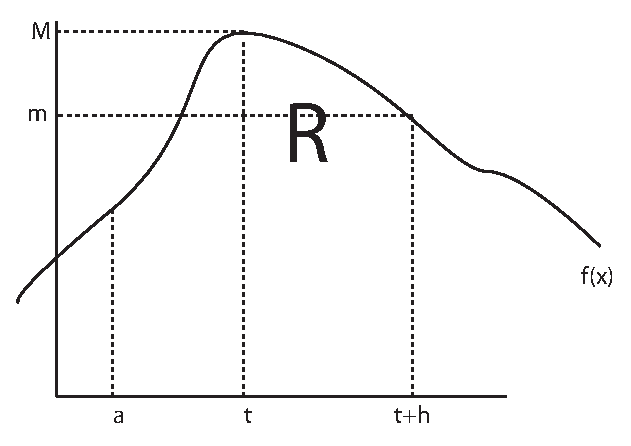
\epsfig{file=fundamental.eps, scale=.5}
\end{center}

As $h\rightarrow 0$ we have $m\rightarrow f(t)=M$. \pause Thus,

$$m\leq \frac{F(t+h)-F(t)}{h}\leq M$$ \pause implies that $$\lim_{h\rightarrow 0} \frac{F(t+h)-F(t)}{h} =f(t)$$
or that $$F^\prime(t)=f(t) \hspace{.2in }\Box$$

\end{frame}



\begin{frame}
\frametitle{Fundamental Theorem of Calculus}

\begin{theorem}
Proposition: If $g$ has a continuous derivative, then $$\int_a^b g^\prime(x)=g(b)-g(a)$$
\end{theorem} \pause

\end{frame}


\begin{frame}
\frametitle{Fundamental Theorem of Calculus}

Proof: Let $$H(t)=g(t)-\int_a^t g^\prime(x) dx$$ \pause
Then $$H^\prime(t)=g^\prime(t)-g^\prime(t)=0 \hbox{ for all } t$$ \pause
Therefore $H$ is a constant, and $H(a)=H(b)$ for all $a, b$.  $$H(a)=g(a)-\int_a^a g^\prime(x) dx= g(a)$$ 
\pause and since $H(a)=H(b)$, it must be that $H(b)=g(a)$ also. 

\pause Therefore
$$g(a)-\int_a^a g^\prime(x) dx=g(b)-\int_a^b g^\prime(x) dx, \hbox{ or} $$ $$\int_a^b g^\prime(x)=g(b)-g(a) \hspace{.1in}\Box$$

\end{frame}



\begin{frame}
\frametitle{Apply Fundamental Theorem of Calculus}

\begin{eqnarray}
\int_{a}^{b} f^{'} (x) dx & = & f(b) - f(a) \nonumber 
\end{eqnarray} 

\begin{itemize}
\item[-] Calculate \alert{antiderivative}
\item[-] Evaluate at $b$
\item[-] Evaluate at $a$
\end{itemize}

\end{frame}



\begin{frame}
\frametitle{Some Classic Antiderivative Formulas} 

\alert{antiderivative} = \alert{indefinite integral}
\begin{eqnarray}
\int 1 dx & = &  x + c \nonumber \\
\int k dx & = & k x + c \nonumber \\
\int x^{n} dx & = & \frac{x^{n+1}}{n + 1} + c \nonumber \\
\int \frac{1}{x} dx & = & \log x + c \nonumber \\
\int e^{x} dx  & = & e^{x} + c \nonumber \\
\int a^{x} dx & = & \frac{a^{x} } {\log a }  + c \nonumber 
\end{eqnarray}

\end{frame}



\begin{frame}
\frametitle{Example 1: Uniform Distribution}

Suppose $f: R \rightarrow R$, with 

\begin{eqnarray}
f(x) & =&  1 \text{ if  } x \in [0,1] \nonumber \\
f(x) & = & 0 \text{ otherwise } \nonumber
\end{eqnarray}
\pause 

What is the area under $f(x)$ from $[0, 1/2]$? \pause \\
\begin{eqnarray}
\int_{0}^{1/2}  f(x)dx & = & \int_{0}^{1/2} 1 dx \nonumber  \pause \\
							& = & x|_{0}^{1/2} \nonumber  \pause \\
							& = & (1/2) - (0 ) \nonumber \\
							& = & 1/2 \nonumber 
\end{eqnarray}
\pause 

We will call $f(x) = 1$ the uniform distribution.   

\end{frame}

\begin{frame}
\frametitle{Example 2: Area Under a Line} 

Suppose $f: R \rightarrow R$, with 

\begin{eqnarray}
f(x) & = & x \nonumber 
\end{eqnarray}

\pause 

Evaluate the $\int_{2}^{t}f(x)dx$  \pause 
\begin{eqnarray}
\int_{2}^{t}f(x)dx & = & \int_{2}^{t} x dx \nonumber  \pause \\
						& = & \frac{x^{2} }{2} |_{2}^{t} \nonumber  \pause  \\
						& = & \frac{t^2}{2} - \frac{2^2}{2} \nonumber  \pause \\
						& = & \frac{t^2}{2} - \frac{4}{2} = \frac{t^2}{2} - 2 \nonumber 
\end{eqnarray}						

\end{frame}



\begin{frame}

\begin{itemize}
\item \textcolor{mygray}{Integral}
\item \textcolor{mygray}{Fundamental Theorem of Calculus}
\item \textcolor{myblack}{Integration Facts}
\item \textcolor{mygray}{Indefinite and Definite Integrals}
\end{itemize}

\end{frame}



\begin{frame}
\frametitle{Integration Facts}

\begin{thm} If $f_{1}, f_{2}: [a,b] \rightarrow \Re$ and $f_{1}, f_{2} $ are integrable on [a,b], then
\begin{itemize}
\item[i)] Consider the interval $[a,b]$ and $c \in [a,b]$.  Then, 
\begin{eqnarray}
\int_{c}^{c}f^{'}_{1}(x) dx & = & f_{1}(c) - f_{1}(c) = 0 \nonumber \\
\int_{a}^{b} f^{'}_{1} (x) dx & = & \int_{a}^{c} f^{'}_{1} (x) dx + \int_{c}^{b} f^{'}_{1}(x)dx \nonumber \\
										& = & (f_{1} (c) - f_{1}(a) +  (f_{1}(b) - f_{1}(c) ) \nonumber \\
										& = & f_{1}(b) - f_{1}(a) \nonumber 
\end{eqnarray}										  
\end{itemize}

\end{thm}

\end{frame}



\begin{frame}
\frametitle{Integration Facts}

\begin{thm} If $f_{1}^{'}, f_{2}^{'}: [a,b] \rightarrow \Re$ and $f_{1}^{'}, f_{2}^{'} $ are integrable on [a,b] and $f_1^{'}$ has antiderivative is $f_1$ and $f_2^{'}$ has antiderivative $f_2$, then
\begin{itemize}
\item[ii)] For $c_{1}, c_{2} \in \Re$ then
\begin{eqnarray}
\int_{a}^{b} (c_{1} f_{1}^{'}(x) + c_{2} f_{2}^{'}(x) ) dx & = & c_{1} \int_{a}^{b} f_{1}^{'}(x)dx  + c_{2} \int_{a}^{b}f_{2}^{'}(x) dx \nonumber 
\end{eqnarray}
\end{itemize}
\end{thm}

\end{frame}



\begin{frame}

\begin{itemize}
\item \textcolor{mygray}{Integral}
\item \textcolor{mygray}{Fundamental Theorem of Calculus}
\item \textcolor{mygray}{Integration Facts}
\item \textcolor{myblack}{Indefinite and Definite Integrals}
\end{itemize}

\end{frame}



\begin{frame}
\frametitle{Indefinite Integrals}

\ \\If $g(x)$ is a primitive of $f(x)$ (so that $g^\prime(x)=f(x)$), then the set of all primitives of $f(x) $ is the set of all functions of the form $g(x)+C$, where $C$ is any constant.  $C$ is known as the \textit{constant of integration} \pause

\ \\Let $f(x)=x+7$; we know that a primitive of $f(x)$ is $g(x)=\frac{1}{2} x^2 + 7x$ \pause

\ \\It's also the case that $\tilde{g}(x)=\frac{1}{2} x^2 + 7x+23$ is a primitive of $f$ \pause

\ \\Given a function $f$, the set of \textit{all} its primitives is the \textit{indefinite integral} of $f$, and is written $$\int f(x) dx$$

\end{frame}



\begin{frame}
\frametitle{Indefinite Integrals: Examples}

Example: The indefinite integral  $\int 12x^2 dx=4x^3+C$, where $C$ is an arbitrary constant \pause

\begin{itemize}
\item[1] $$\int x^\alpha dx = \frac{1}{\alpha+1} x^{\alpha+1}+C \hbox{ if }\alpha\not=-1$$ \pause

\item[2] $$\int \frac{1}{x} dx=\ln x+C $$ \pause

\item[3] $$\int e^x dx =e^x +C$$
\end{itemize}

\end{frame}



\begin{frame}
\frametitle{Indefinite Integrals: Examples}

\begin{itemize}
\item [1'] $$\int (x-a)^\alpha dx = \frac{1}{\alpha+1} (x-a)^{\alpha+1}+C \hbox{ if }\alpha\not=-1$$ \pause

\item [2'] $$\int \frac{1}{x - a} dx=\ln (x-a)+C \hbox{ if }x>a$$ \pause

\item [3'] $$\int e^{ax} dx =\frac{e^{ax}}{a} +C$$ 
\end{itemize}

\end{frame}



\begin{frame}
\frametitle{Definite Integrals}

\ \\With definite integrals we do not need to worry about the constant of integration: \pause We know that $$\int_a^b g^\prime(x) dx=g(b)-g(a)$$ \pause If we used $g(x)+C$ as our primitive instead we'd get \pause $$\int_a^b g^\prime(x) dx=(g(b) +C)-(g(a)+C)=g(b)-g(a)$$


\end{frame}

\end{document}
